\documentclass[tikz,dvipsnames]{standalone}

\begin{document}

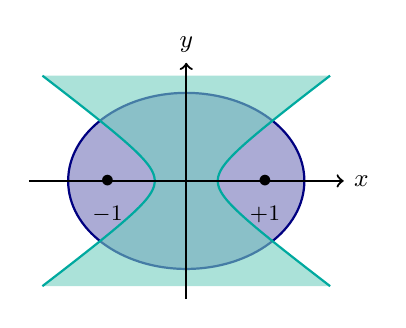
\begin{tikzpicture}
    \filldraw[color=NavyBlue,thick,fill=NavyBlue!55,fill opacity=0.6] (0, 0) ellipse (1.5cm and 1.118cm);

    \pgfmathsetmacro{\a}{0.8}
    \pgfmathsetmacro{\e}{1.25}   % eccentricity
    \pgfmathsetmacro{\b}{\a*sqrt((\e)^2-1)}
    \path[fill=Emerald!55,opacity=0.6]
    plot[domain=-2.2:2.2] ({\a*cosh(\x)/2},{\b*sinh(\x)/2})
    --plot[domain=2.2:-2.2] ({-\a*cosh(\x)/2},{\b*sinh(\x)/2})--cycle;
    \draw[scale=0.5,color=Emerald,smooth,thick,variable=\x] plot[domain=-2.2:2.2] ({\a*cosh(\x)},{\b*sinh(\x)});
    \draw[scale=0.5,color=Emerald,smooth,thick,variable=\x] plot[domain=-2.2:2.2] ({-\a*cosh(\x)},{\b*sinh(\x)});
    
    
    \node[label=below:\footnotesize{$-1$}] (a) at (-1,0) {$\bullet$};
    \node[label=below:\footnotesize{$+1$}] (b) at (1,0) {$\bullet$};
    \draw[->,thick] (-2,0)--(2,0) node[right]{\small{$x$}};
    \draw[->,thick] (0,-1.5)--(0,1.5) node[above]{\small{$y$}};
    \end{tikzpicture}

\end{document}